\section{Our Analysis}

In this section, we will analyze the details of each onion design. As we stated before, Based on those analysis, we propose backup strategies for each data type accordingly. Intuitively, the strategy is to the find the smallest onion to backup and recover. In this discussion, we will focus on backup for each column, and the situation for a table should be the same. 
% The onion 'search' for string is not yet implemented in the newest version of CryptDB, so for this onion, our analysis is based on the description in \citep{song2000practical}.

In CryptDB, each column in a table can be encrypted into several onions. Each onion can have several layers. We have to make a choice whether to remove or retain a onion. If one column has three onions, we will have eight choices. Since we can not remove all of the onions, there are seven possible choices. For each onion, we can either choose to backup it directly, or to decrypt some layers and then backup it. We will discuss whether those choices are practical.

\begin{figure}[tb]
\centering
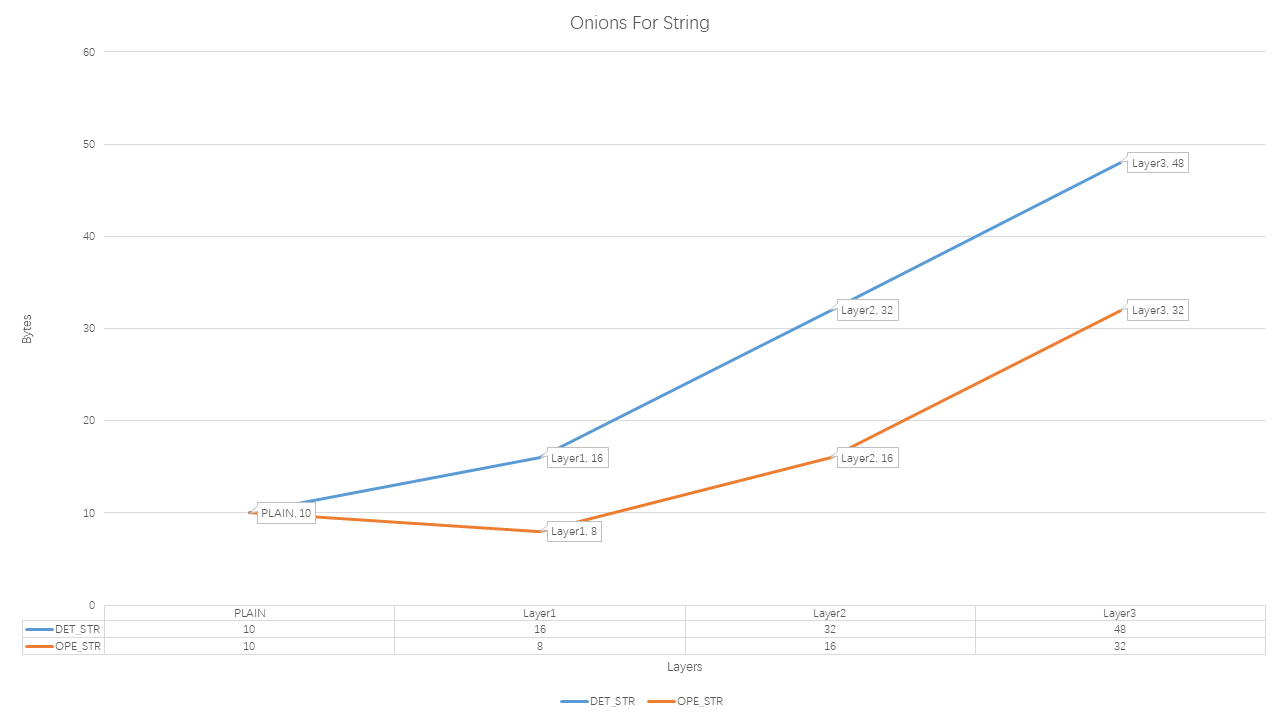
\includegraphics[width=\columnwidth]{images/onions-for-string.png}
\caption{onions-for-string}
\label{fig:stack4}
\end{figure}


\begin{figure}[tb]
\centering
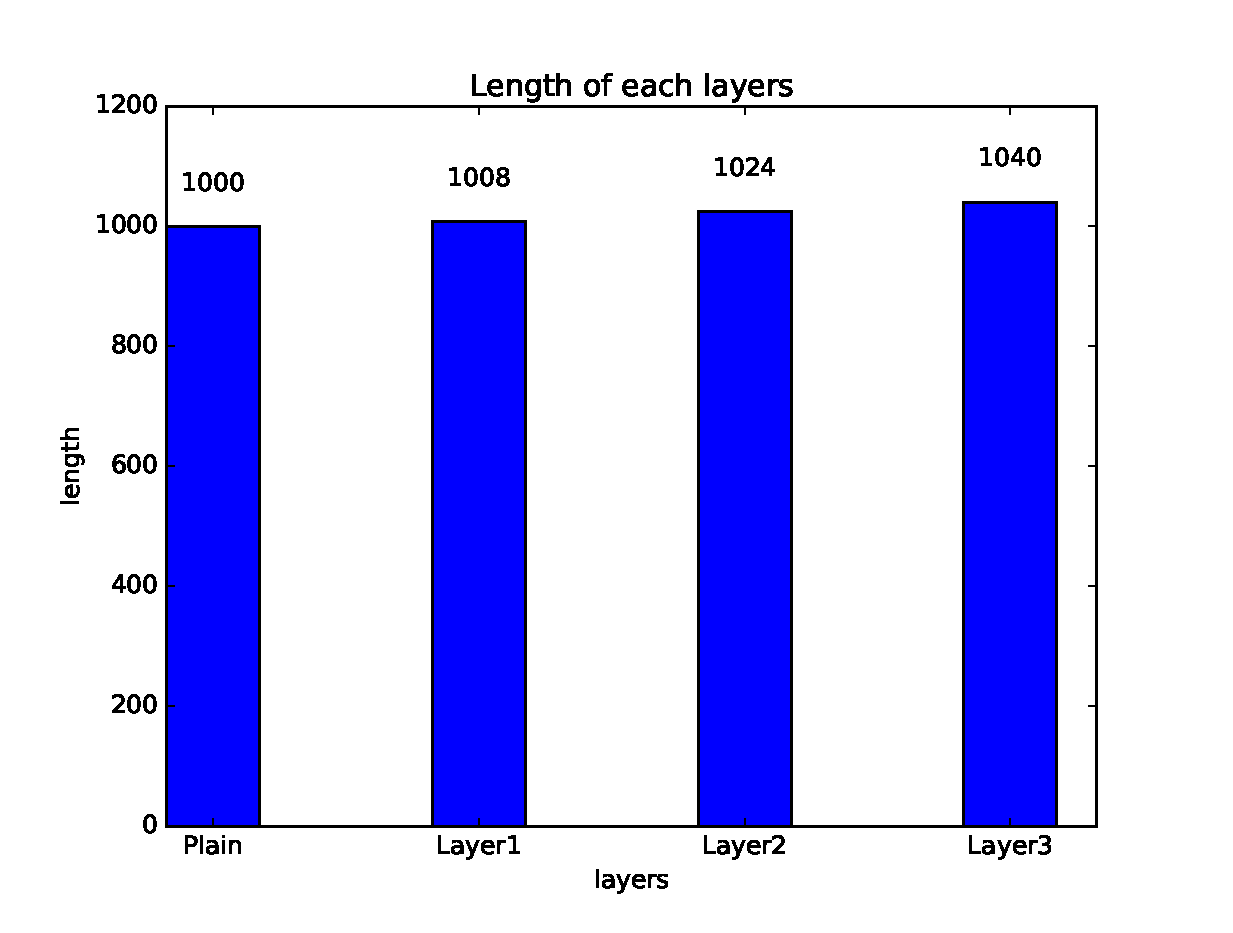
\includegraphics[width=\columnwidth]{images/det_str.eps}
\caption{det-str-eps}
\label{fig:stack5}
\end{figure}



Figure~\ref{fig:stack4},~\ref{fig:stack5} shows how the size of a string change for each onion and each layer of the onions. As the figure depicts, for the onion DET, the plain text is 10 Bytes long, while the size of the onion in layer RND is 48 Bytes long. That because the onion DET has three layers, namely DET-JOIN, DET, and DET-RND. The first two layers uses AES-CMC for encryption, and the third layer uses AES\_CBC. In the current implementation, block size of 16 bytes is uses. In current version of CryptDB, the input text of the algorithm can not be divided exactly by the block size, then the input should be padded with zero to make it divisible. If the input text is divisible, cryptdb will pad the text by one block. So, for plain text with size 10 Bytes, after it is encrypted with layer DET-JOIN, it becomes 16 Bytes. After it is encryptdb with layer DET, it is padded to 32 Bytes. And when it is in layers DET-RND, the size becomes 48 Bytes. Note that for ciphertext, CryptDB used only the integer type of MySQL if the size of ciphertext can fit in that data type. Otherwise, varbinary is used instead. Since Onion Search is not implemented properly, we do not include it in the figure. In fact, the onion search is quiet simple: it has only two layers, and according to \citep{song2000practical}, the size of ciphertext is roughly the same as plaintext. In the current implementation, the change of data type and size of OPE is quiet complex. In fact, the Onion OPE only guarantee the properity of order preserving for 8 bytes prefix of a string.




\begin{figure}[tb]
\centering
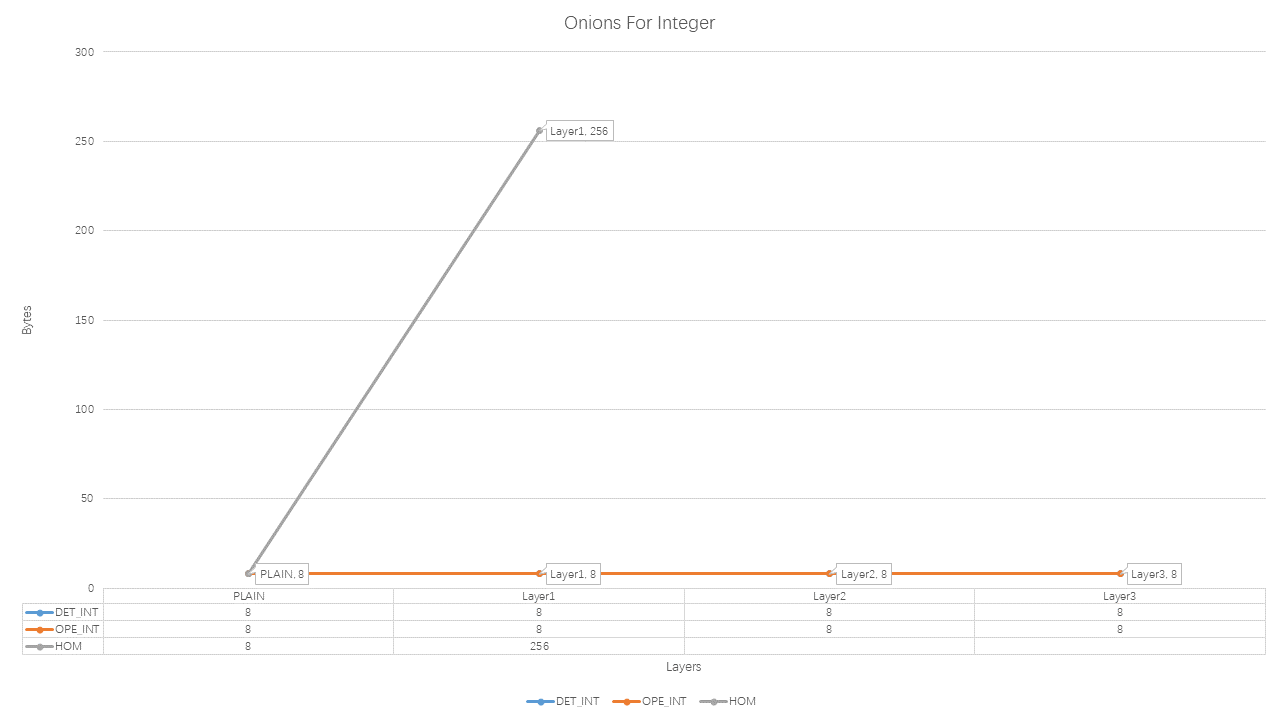
\includegraphics[width=4cm]{images/onions-for-integer.png}
\caption{onions-for-integer}
\label{fig:stack6}
\end{figure}


Figure~\ref{fig:stack6} shows how the storage size change for each onion for integer type. Currently, there are three onions for integer, HOM uses Pailliar algorithm, DET for integer uses 64bits blowfish, so the size of the ciphertext is always 64bits integer. There is no padding. HOM uses pailliar, so the result is always 256bytes integer. MySQL do not has such long integer, so varbinary(256) is used instead. Now let's discussion how the size change across layers of the onion OPE for both String type and Integer type. 



OPE requires that the cipher text size is double the size of plain text. Let's first discuss OPE-INT. This onion has three layers, namely OPE-INT-JION,OPE-INT,OPE-RND. If the plaintext is of the type tinyint, which has only 1 Bytes. Then after the layer OPE-INT-JOIN, it becomes 2 Bytes, and after the layer OPE-INT, it becomes 4 Bytes. So for the layer OPE-RND, the input is a 4 Bytes long integer, and the result of OPE-RND can be represented by a 8 Bytes bigint in MySQL. If the size of the integer is 64 bits, then after the encryption of one layer of OPE, the ciphertext should be 128 bits, which can not fit in an integer type. Cryptdb uses 128 bits varbinary data type. In that case, the input of the layer rnd is string instead of integer, so algorithm AES is used instead of blowfish. So the onion OPE-INT may contain layer RND-STR. 

Then let's talk about OPE-STR. OPE-STR can also have three layers, OPE-STR-JOIN, OPE-STR, OPE-RND. When the input of the algorithm is a string, plaintext length of 4 Bytes and  ciphertext length of 8 Bytes are specified. That is, only the prefix are encrypted and has the properity of order preserving. Then in the layer OPE-STR, since in the first layer, the data type has been transformed to 64bits integer, the OPE-STR is transformed to OPE-INT, and the input is 64bits long. So after this layer, integer can no longer fit ciphertext. The data type has become 128 bits varbinary type. And then in the third layer, aes is used for the layer, adding one block to the size, making the total size of the onion 32 Bytes.


The above discussion reveals two facts:

\begin{itemize}
\item[--] The size of Onion OPE can not exceed 32 Bytes regardless of the size of plaintext
\item[--] Onion OPE can loose information of the plaintext, so we can not use the Onion OPE
\end{itemize}



As we have known the property of the encryption schemes and the data layout. We can now start to design the strategy of deduplication. We will first discuss each onion and then give three simple strategies for analysis. Then in the experiment section, we will use our workload to test the strategies. We first discuss the design choices for each onion of interger data and string data. 


\begin{itemize}
\item Integer/String OPE: For ope-int, we have little choices, since OPE is not able to be decrypted. If this onion is removed, then we need two OPE-Encrypt operation and one AES-enctypt operation to get it back. 
\item Integer HOM: HOM takes a long time to recover, and also occupy 256 Bytes. If we choose to remove it, we should use one Paillar-encrypt operation to get it back. Only retaining HOM is never a good choice, because it takes a long time to decrypt HOM for recovery, and also the storage size is large. So HOM should be removed or be retained together with other onions.
\item Integer/String DET: If this onion is removed, then it takes three blowfish-encrypt operations to recover it. For String type, we need two AES-CMC-encrypt and one AES-CBC-encrypt operation to recover the onion. The encryption time is related to the size of the string.
\item Integer IV: 8Bytes integer. faster to regenerate
\end{itemize}



Since the detailed performance is related to so many things, we do not provide exact strategy for backup. Instead, we summarize several Principals for cryptdb backup and then give some examples. 

\begin{itemize}
\item[--] One original field is replicated several times and encrypted with different schemes
\item[--] If we want mininum storage overhead, then for each field we can find the onion with the least size, like AES or blowfish, that can produce ciphertext of the size similar to plaintext, and remove all other onions. If we want minimum time overhead, we should backup all the onions, so that we can recover the data directly. Other choices are something in between.
\item[--] Metadata should have a full backup for data recovery, and the size of metadata is small. 
\item[--] For recovery, we need to decrypt the onion we have, and based on the metadata, recompute the ciphertext for other onions.
\item[--] For one onion, we can choose the stay in RND layers, which means identical plaintext can have different ciphertext. If we decypt it to a layer that is not random, then identical plaintext can have the same ciphertext. If most of the plain text in this column are the same, then it will be easy to compress this filed to reduce storage overhead. Also, if we decrypt RND layer, then we can remove the IV column, which further reduces storage overhead.
\end{itemize}


Based on the principals, we proposes the following strategies for String data and Integer data. 

\begin{itemize}
\item[--] Remove RND and use DET onion will produce the least storage overhead.
\item[--] Do not remove anything. This is the strategy with the most storage over head and least computation overhead
\item[--] Retain RND and salt for DET, remove HOM and OPE, and Search. This method has high security level.
\end{itemize}




For those two data types and strategy, we construct microbenchmark to do experiments. Actually, the time needed for recovery can be reduced by using multi-threading or other optimization. We assumes that other factors are the same and only condiser the overhead of recomputation. We use single thead whith pipeline insert.

So, the overall strategy looks like the following: we let users choose the strategy bases on the what they care about. They can either choose to backup all the onions, or choose to have minimum backup or something in between. Figure~\ref{fig:stack7} and Figure~\ref{fig:stack8} shows how to encrypt and extend the plain text, and then choose one onion for back up, and then compress the onion. For recovery, we should first decrypt the onions and then recompute the deleted onion. Then we should be able to construct the sql queris for recovery. This is the same as the logical backup recovery method.

\begin{figure}[tb]
\centering
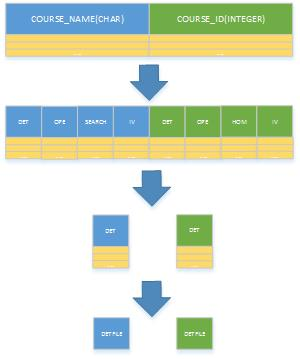
\includegraphics[width=4cm]{images/Workflow.jpg}
\caption{Backup and compression}
\label{fig:stack7}
\end{figure}


\begin{figure}[tb]
\centering
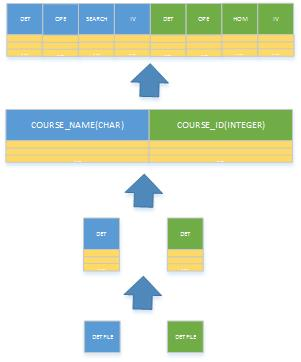
\includegraphics[width=4cm]{images/Recovery.jpg}
\caption{Aes encryption and decryption time}
\label{fig:stack8}
\end{figure}
